%\section{The \gls{mSTS} as the pathfinder for the STS}
The mCBM~\cite{mCBM} is considered a FAIR Phase 0 experiment and the precursor of the \gls{CBM}. The first mCBM campaign took place in 2019 after two years of preparations in the detector test area HTD \cite{progress_report_2017_sturm}. The first \gls{mSTS} prototype was operated together with mTRD, mTOF, mRICH, and mPSD, and it consisted of one tracking station, 4 detector modules (8 \gls{FEB}s mounted onto two carbon ladders, and then subsequently in two C-frames. The next iteration of the \gls{mSTS} features 11 detector modules, and it was assembled in order to have a better understanding of the components and the performance of a more complex structure. Completing 11 modules (together with the QA procedures, testing of the STS-XYTERs and \gls{FEB}s), readout, and control software, set an important milestone on the way to the STS. The first section of this chapter gives an overview of the mCBM experiment and focuses on the DCS architecture and gives an introduction to the detector operation. The next sections summarize the assembly of the \gls{mSTS} and its hardware. At last, the results obtained through DCS will be discussed. 

\section{mCBM the phase 0 experiment}
The mCBM aims to test and optimize the performance of the detectors including crucial software and hardware components. The experiment uses beams from SIS18 synchrotron at energies up to 2 AGeV and intensities up to $10^{9}$ ions/s. The test setup is positioned downstream of a solid target with a polar angle of about \SI{25}{\degree} (see figure~\ref{fig_mcbm}).

\begin{figure}[!h]
\centering
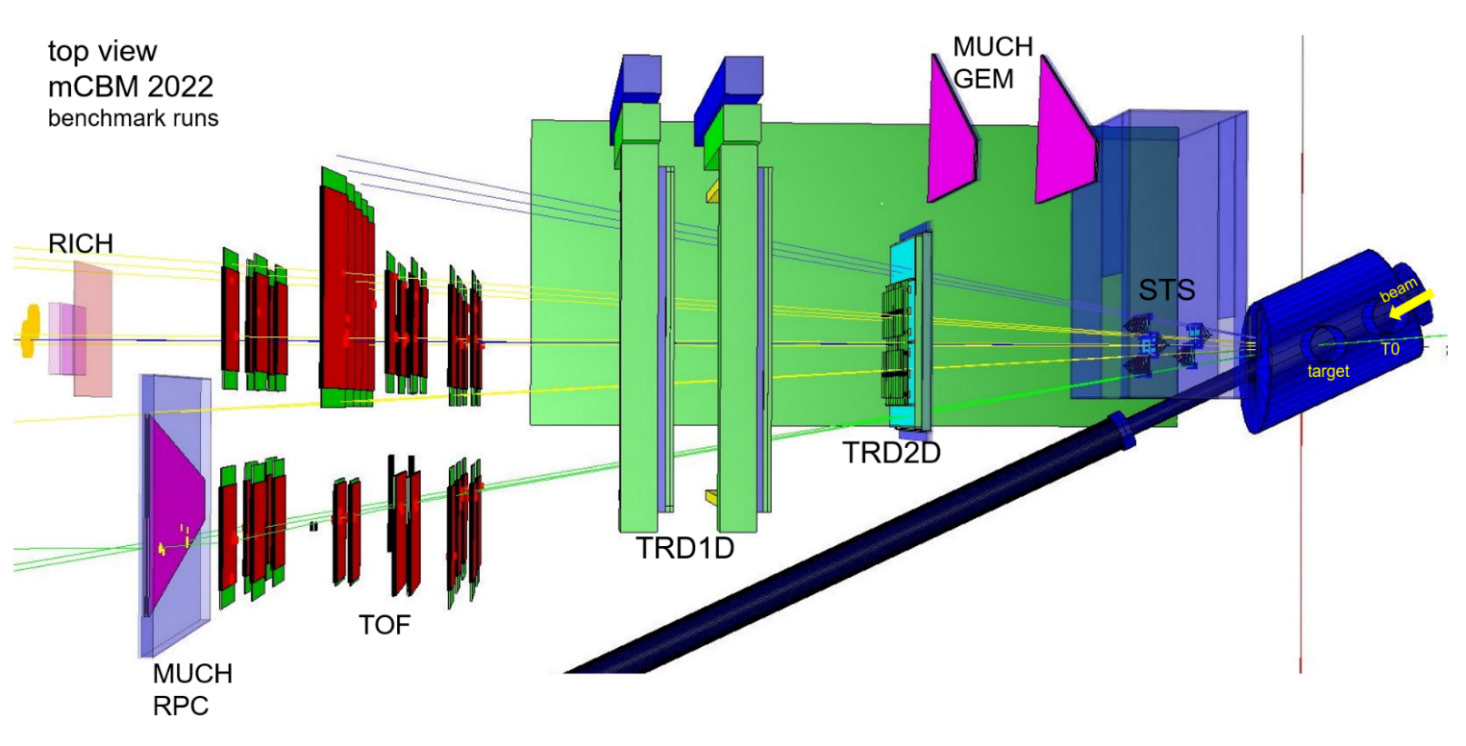
\includegraphics[width=0.7\columnwidth]{Chapter5/DCS/images/mcbm_2021_setup.png}
\caption{Schematical view of the mCBM experiment in 2022}
\label{fig_mcbm}
\end{figure}

The developments of DAQ, First Level Event Selector (\gls{FLES}), or \gls{DCS} will significantly reduce the commissioning time required for the CBM experiment at the SIS100 synchrotron. The mCBM \gls{DAQ} is based on the common readout interface (\gls{CRI}) (see section \ref{DAQ}). Each subsystem uses up to a few CRI boards. Apart from exercising the readout chain and DCS, the mCBM aims to operate the subsystems in the high-rate nucleus-nucleus collision environment. The development of the readout chain has a significant role, in order to be able to improve the free streaming data acquisition and transport to the computer farm. Moreover, offline data analysis, online tracking, event reconstruction, and event selection algorithms have been intensively investigated. 

\begin{figure}[!h]
\centering
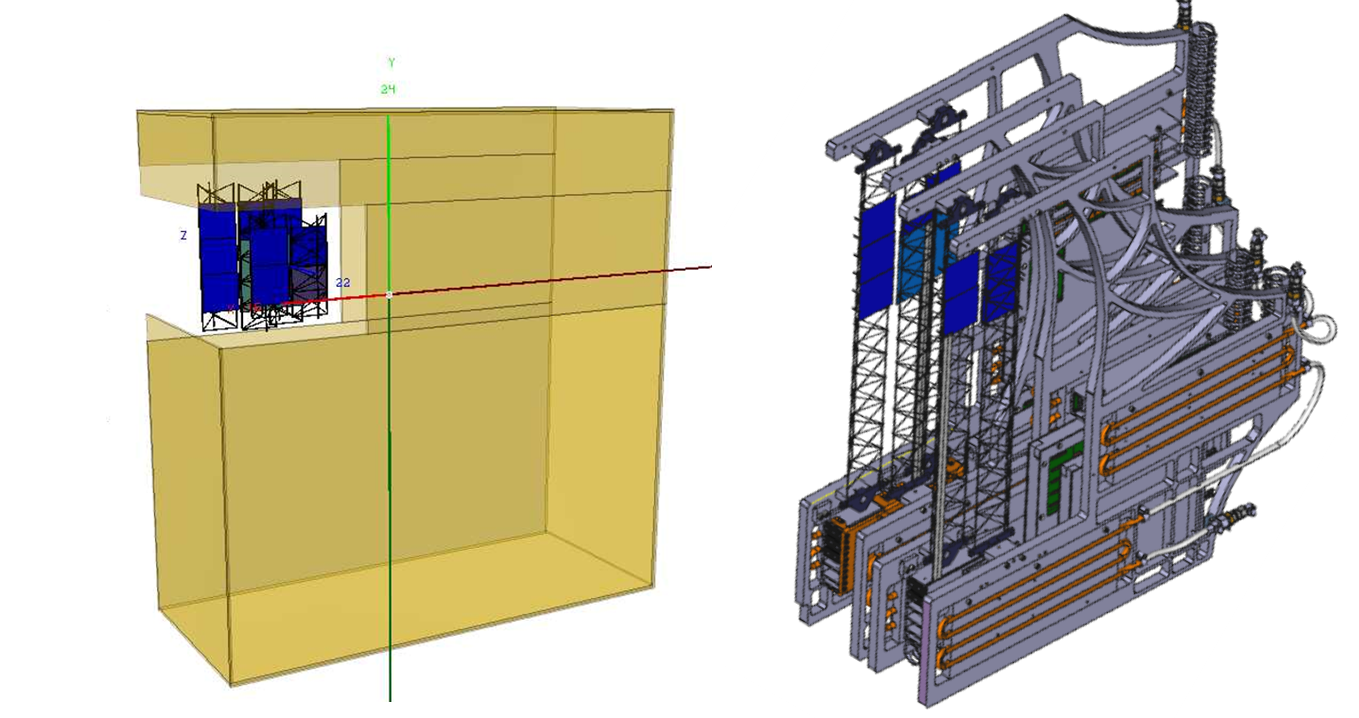
\includegraphics[width=0.75\columnwidth]{Chapter5/DCS/images/mSTS_mech.png}
\caption{Mechanical design (right) and simplified geometry of the \gls{mSTS} together with its enclosure (left)}
\label{fig_STS}
\end{figure}

Figure~\ref{fig_STS} depicts the latest \gls{mSTS}, which features 4 units forming 2 tracking stations of 5 ladders, 11 modules, 24 \gls{FEB}s (22 readout \gls{FEB}s + 2 pulser \gls{FEB}s), and 176 readout \gls{ASIC}s. The mentioned pulser \gls{FEB}s are additional boards that are triggered by the beam and were added to the system as a time reference and to check the data flow in the system.  Most of the components used for the assembly of the detector are close to the final ones, therefore the operation of the \gls{mSTS} gives us a perfect opportunity to study the modules in detail.
\subsection{Data-taking campaigns}
After the commissioning of the new \gls{mSTS} experiment in June 2021, the first data-taking took place in July featuring collisions of oxygen on a nickel target at 2.00 AGeV with intensities of $10^{10}$ ions/spill. The spill duration was set to \SI{10}{seconds}, therefore effective intensity reached $10^{9}~\mathrm{ions/s}$. This campaign allowed performing last checks of the DCS and other systems, before the announced $\Lambda$ benchmark runs in 2022 \cite{sturm3}. During that beam campaign, great spatial and time resolution were confirmed. Moreover, a clear distinction between noise and MIP position was seen. The vertex reconstruction was completed using the correlations of \gls{mSTS} findings. Hit reconstruction efficiency of 97.5\% was achieved, which is consistent with the expectation from models, using the mTOF as an additional external reference~\cite{dario1}. The preceding runs with uranium beams and gold target ($T = 1$ AGeV and average collision rate of 400 kHz) took place in March 2022. The benchmark runs with Ni + Ni ($T = 1.93$ AGeV and average collision rate of 200-300 kHz) were realized in June 2022. During the data taking with the heaviest systems, the silicon sensors were exposed to a significant particles flux, what will be discussed in the next sections. 
\section{Introduction to the detector control}
The next sections give an overview of the control system and used applications. The \gls{mSTS} detector uses most of the container related developments including Phoebus, alarm-system, alarm-logger, Elasticsearch, Kibana, Archiver, Redis \gls{DB}, and the underlying stream-processing platform. The mCBM's subdetectors require control systems but the devices used for the Phase-0 experiment are in most cases different than for the final experiment, therefore efforts toward the DCS will have to be intensified as the final systems will be close to completion. Therefore, the prototyping of the DCS refers mostly to the software components that could be maintained and used during the commissioning and operation of the future experiment. As described in the chapter~\ref{EPICS}, the network serves as a medium allowing a server and client to publish and subscribe to process variables. Those variables are distinguished by its name and follow a certain convention.
\subsection{Nomenclature}
The naming convention should clearly define the detector's place and its functions. A record comprises a record name and aliases that help to identify the variable. In a general case the naming convention is organized into the following specifiers with a colon as a delimiter:
\begin{enumerate} 
\item Experiment: CBM
\item Subsystem: STS
\item Service: Air Drying/Powering (Optional)
\item Location: Unit/Ladder/FEB
\item \gls{FEB} service: high voltage/low voltage
\item Value abbreviation: e.g. IMon/VMon
\end{enumerate}

For example (the first line represents the name and the second one the alias):
\begin{verbatim}
CBM:STS:1:0:2:HV:MeasureCurrent
CBM:STS:11111:5:1:MeasureCurrent
\end{verbatim}
The first line of the example above points to a defined place and functionality in the detector - the current of the HV channel of the given \gls{FEB}. The second line indicates the channel in the power supply module which is being used. This naming convention is then followed by the other services - low voltage power, cooling, etc.  
\subsection{Network structure}
There are three main networks in the mCBM experiment. The first one so-called detector network allows monitoring and control of hardware connected to the respective subsystem. All \gls{DCS} infrastructure, including the main node, is located in that network. The second network "FLES network" is focused only on the data coming from the detectors. The third network is dedicated to the operators and data-taking operations. All these networks are interconnected via gateways.  

\subsection{mSTS's detector control system}
A breakdown of the \gls{mSTS}'s \gls{DCS} architecture is presented in Figure~\ref{fig_mstsarch}. The supervisory layer features several nodes: 2 \gls{SBC}s and two main nodes - the control and archiver node. The first one of the main nodes takes care of the control and monitoring of the whole system (all the containers and applications), and the second node serves as a backup and archiving node. The control layer comprises all the necessary \gls{IOC}s and underlying nodes. The last layer (field layer) features all readout boards, sensors, power supplies, cooling units, etc. The system sums up to about 5000 process variables and about 10\% of them need to be archived. Moreover, the control system software (containers, \gls{IOC}s) needs to be also monitored, in order to detect any kind of malfunction. 

\begin{figure}[!h]
\centering
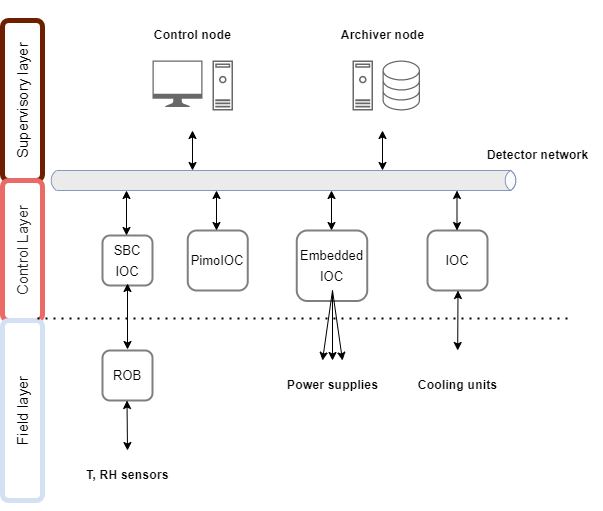
\includegraphics[width=0.55\columnwidth]{Chapter5/DCS/images/mcbmpng.png}
\caption{A general structure of the \gls{mSTS} DCS architecture}
\label{fig_mstsarch}
\end{figure}

\subsection{Finite state machine and its role}
The \gls{mSTS} as opposed to the final STS doesn't require sophisticated hardware and software interlocking mechanisms. The biggest risk to the safe operation are:
\begin{itemize}
    \item too high temperature (exceeding \SI{60}{\degreeCelsius})
    \item ambient temperature reaching dew point 
    \item sudden loss of cooling unit (e.g. due to radiation-induced damage)
    \item high leakage current (usually too high currents are managed by the trip conditions of the power supply)
\end{itemize}
A proposed \gls{FSM} for the \gls{mSTS} can be seen in the figure~\ref{fig_FSM}. Each state of the \gls{FSM} represents a well-defined detector state. After initialization of all the services, the detector enters into the standby state, in which the cooling stabilizes and the detector is in a safe state. Next transitions and stages prepare the \gls{mSTS} for the operation and data taking, low voltage and subsequently high voltage channels are turned on. In case any of the issues listed above happens, the detector is brought into a safe state (error state), which in most cases requires operator intervention. The global states mentioned to the right of the block diagram are the states propagated to the higher levels of control (\gls{SCA}/\gls{ECS}).
\begin{figure}[h!]
\centering
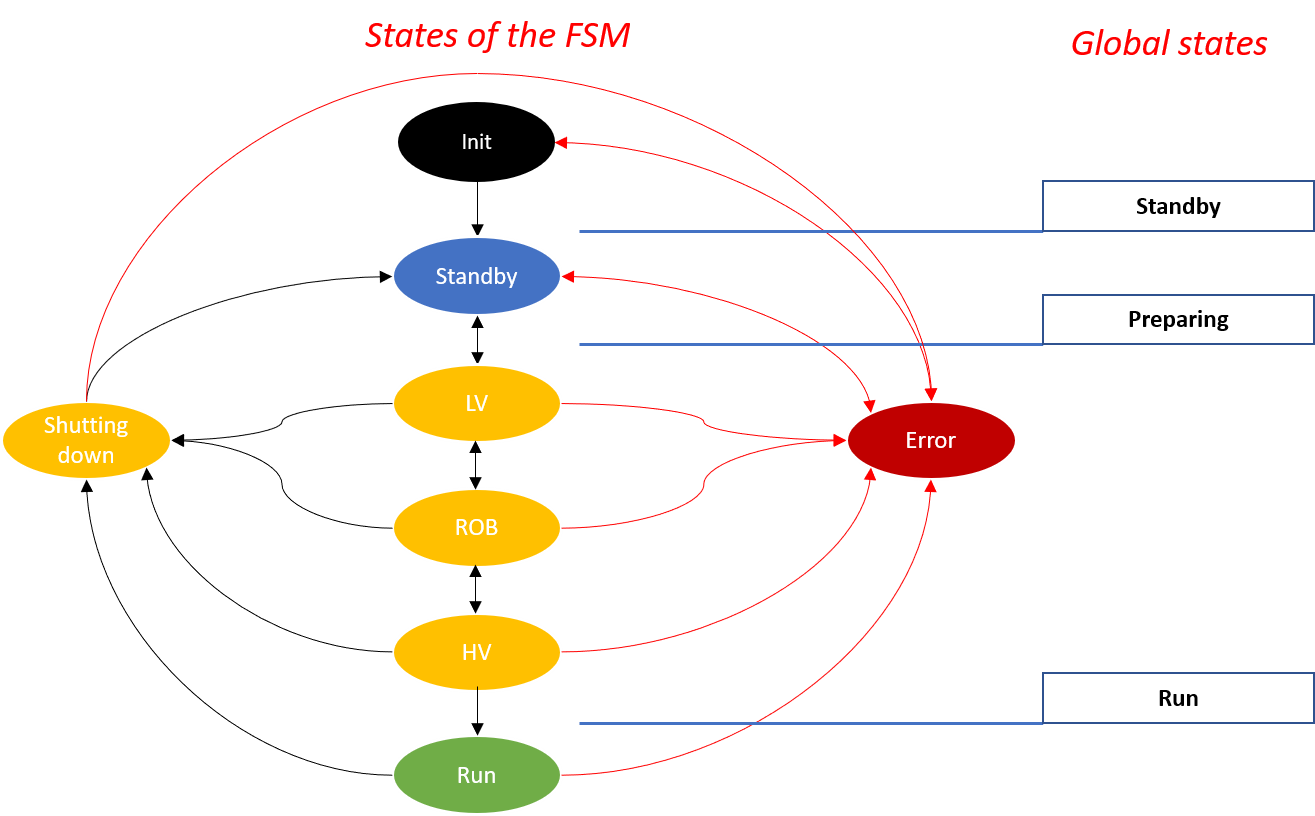
\includegraphics[width=0.8\columnwidth]{Chapter5/DCS/images/FSM.png}
\caption{Proposed finite state machine for the \gls{mSTS}}
\label{fig_FSM}
\end{figure}

\newpage
\subsection{Containers monitoring - Weavescope}

Weave Scope is a visualization and monitoring tool for Docker and Kubernetes. It offers a detailed view into the applications as well as your entire infrastructure and allows you to diagnose any problems with your distributed containerized-time real-time, as it is being deployed to a cloud provider. Weavescope has proved to be a useful tool for running commands and configuring the containers after their initialization. The container publishes the values from the chillers, hence the container is connected to Phoebus, archiver, alarm-server, and sequencer. 
%\begin{figure}[!h]
%\centering
%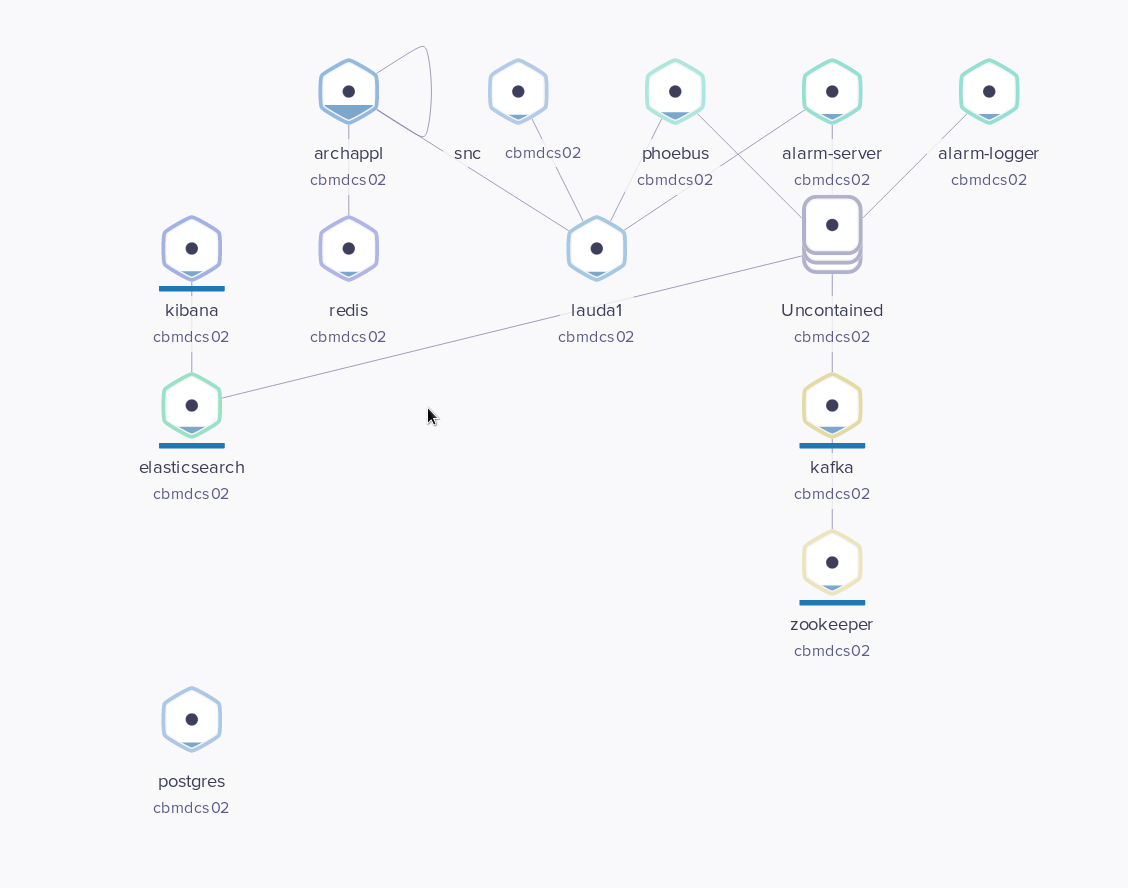
\includegraphics[width=0.55\columnwidth]{Chapter5/DCS/images/weave.png}
%\caption{mSTS - weavescope view}
%\label{fig_weave}
%\end{figure}
%\newpage
\subsection{IOC monitoring - heartbeat and PIMO}
Apart from container monitoring, the \gls{IOC}s database contains also a heartbeat record which gives an indication of whether it's working properly. Moreover, an additional tool called PIMO \gls{IOC} was deployed. It's a ping monitor, which indicates whether a given \gls{IOC} is reachable in the network. Losing an \gls{IOC} would indicate an error. When it comes to machine safety, \gls{mSTS}'s \gls{FSM} should also react to the disconnection of PVs which are being monitored.
\subsection{Process variables monitoring and control}
As described also in the figure~\ref{fig_mstsarch}, the three monitoring blocks are: relative humidity and temperature sensors, cooling, and powering. In  order to monitor ambient conditions, 7 PT100 temperature sensors and one relative humidity sensor (Sensiron SHT85) were placed inside the \gls{mSTS}~\cite{SHT85}. Additionally, one sensor was placed outside of the detector enclosure to monitor the temperature in the experiment cave. The temperature sensors were read out using a dedicated readout board connected to a Raspberry PI board which features a \gls{IOC}. Similarly, the humidity sensors were read out by a microcontroller board connected to the same \gls{SBC} and \gls{IOC}.

The control of the \gls{mSTS}'s modules powering is organized twofold. All low voltage and high voltage modules are controlled via CC24 controller~\cite{cc24} inside MPOD crates~\cite{mpod}. Each CC24 controller has an embedded \gls{IOC} which was customized for the system requirements.  An operator can either use the \gls{SNMP} based communication, ca-tools, or a dedicated \gls{GUI}. In the case of SNMP scripts, the user has access to single channels, and specific channel-hardware connection knowledge is required to properly handle the detector. On the other hand, thanks to the aliases assigned to the process variables, specific channels could be switched on (through CA, PVA, or \gls{GUI}) by knowing the position of the \gls{FEB} in the detector. The cooling section will be discussed in section~\ref{msts_cooling}.

%\newpage